\section{Overview}

The diurnal variation of the global electric circuit is investigated using the World Wide Lightning Location Network (WWLLN), which has been shown to identify nearly all thunderstorms (\citet{Jacobson2006c}, using WWLLN data from 2005).
To create an estimate of global electric circuit activity, a clustering algorithm is applied to the WWLLN dataset to identify global thunderstorms from 2010 -- 2013.
Annual, seasonal, and regional thunderstorm activity is investigated in this new WWLLN thunderstorm dataset in order to estimate the source behavior of the global electric circuit.
Through the clustering algorithm, the total number of active thunderstorms are counted every 30 minutes creating a measure of the global electric circuit source function.
The thunderstorm clusters are compared to precipitation radar data from the Tropical Rainfall Measurement Mission satellite and with case studies of thunderstorm evolution.

The clustering algorithm reveals an average of $660 \pm 70$ thunderstorms active at any given time with a peak-to-peak variation of 36\%.
The highest number of thunderstorms occurs in November ($720 \pm 90$) and the lowest number occurs in January ($610 \pm 80$).
Thunderstorm cluster and electrified storm cloud activity are combined with thunderstorm overflight current measurements to estimate the global electric circuit thunderstorm contribution current to be $1090 \pm 70$~A with a variation of 24\%.
By utilizing the global coverage and high time resolution of WWLLN, the total active thunderstorm count and current is shown to be less than previous estimates based on compiled climatologies.

Diurnal variation in global thunderstorm activity was original observed by \citet{Wilson1921} and \citet{Whipple1929} through a combination of thunderstorm day and electric field measurements.
Strong correlations between thunderstorm activity and fair weather return current led to the model of the global electric circuit, a system of ionospheric charging and discharging through thunderstorms and fair weather return currents.
Studies to date have estimated that globally there are 1000 -- 2000 thunderstorms active at any one time, with most concentrated over tropical landmasses, covering 1 -- 10\% of Earth's surface \citep{Markson1978, Rycroft2011a, Singh2011a}.
Previous work on diagnosing the generator source of the global electric circuit used several methods:  long time scales \citep{Tinsley2007, Liu2010}, mathematical models \citep{Kasemir1977, Hays1979, Roble1991}, engineering models \citep{Ogawa1985, Kartalev2004, Rycroft2006}, parameterization \citep{Price1992, Williams1985}, and thunderstorm overflight estimates \citep{Mach2011}.
Most work with the global electric circuit uses long term averaging to recreate the known Carnegie curve of \citet{Whipple1929}, yet short time scales do not match the long term averaging \citep{Holzworth1984a}.
The variation of the global electric circuit changes on short time scales that is not resolved in past models or with long term averaged observations.
The global electric circuit is an important component to the solar-terrestrial system creating a link between solar activity, the ionosphere, aerosols, cloud microphysics, thunderstorms, weather, and climate \citep{Tinsley2007, Holzworth1986}.

Individual lightning strokes and flashes are not yet a reliable method of characterizing the source of the global electric circuit, but global thunderstorm activity is a reliable measure.
\citet{Ruhnke1969} proposes that the displacement current above thunderstorms as the global electric circuit generator source as it varies slowly through the evolution of a thunderstorm and the current is fairly independent from impulsive events like lightning.
\citet{Krider1985} looked at displacement currents below a thunderstorm to find them steady with abrupt, but insignificant, changes due to lightning.
\citet{Rycroft2000c} created an engineering model with three different regions for the the return current, concluding that sprites, lightning, and other transients will have little direct effect on the global electric circuit.
\citet{Stergis1957} showed that cloud to ground lightning is not necessary for upward current from thunderstorms.
With a numerical model of a dipolar thunderstorm \citet{Tzur1985} estimated the average upward current contribution of a thunderstorm to the global electric circuit to be 0.7~A per thunderstorm.
Similarly, with a combination of numerical and analytical models of dipolar thunderstorm, \citet{Driscoll1992} estimated a total contribution of 0.4~A to the global circuit per thunderstorm.
Unlike the other models, \citet{Mareev2008} estimated a 50 -- 400~A current contribution directly from global lightning;  with a similar model \citet{Mallios2012} investigated the efficiency of lightning and found lightning only contributed 1\% (3~A) of the total 300~A contribution from thunderstorms.
These models show that thunderstorms contribute an appreciable upward current to the global electric circuit with a wide range of estimated current contributions.

Balloon and aircraft overflights have been used to estimate the total current contributions from thunderstorms to the global electric circuit.
\citet{Stergis1957} found thunderstorm currents ranging from 0.6 -- 4.3 A, with an average of 1.3 A; these estimates are the lower bound with uncertainties of up to 50\%.
\citet{Blakeslee1989} shows the upward current generated by a thunderstorm to range between 0.1 -- 6~A with an average current between 0.5 -- 1~A.
Other studies show current density over thunderstorms ranging from 10 -- 40 pA/km$^2$ \citep{Holzworth1981} to $-20$ -- 33~nA/m$^2$ \citep{Mach2009}.
The overflights in previous research found no consistent parameterization between lightning rates and fair weather return current, but recent balloon work found strong correlation between global lightning activity and the fair weather return current on short time scales \citep{Holzworth2005}.
Lightning stroke activity and locations cannot directly provide estimates of the global circuit, however they can be used for directly locating and defining active thunderstorm areas and relative intensities.

Compared to satellite and balloon observations, ground based lightning networks have the advantage of continuous observation of large regions.
Global very low frequency networks, such as the World Wide Lightning Location Network (WWLLN), are capable of locating lightning around the entire globe.
\citet{Holzworth2005} compared the stroke counts of a nascent WWLLN to the fair weather return current and found strong temporal correlation between the measurements.
A better measure of global circuit activity is the total number of active thunderstorms around the globe; applying clustering algorithms to lightning network data enables the network to locate, track, and monitor global thunderstorm activity.

The WWLLN data are clustered into thunderstorms with the Density-Based Spatial Clustering of Application with Noise (DBSCAN) algorithm \citep{Ester1996, Kriegel2011a}.
DBSCAN was chosen as the clustering algorithm for several key features: the capability to handle noise, no requirement to specify the number of clusters, arbitrary cluster shapes, and the insensitivity to the ordering of the data.
Clustering lightning strokes into thunderstorms cannot require a designated number of clusters before clustering, as the total number of thunderstorms is not known before clustering.
Similar algorithms, such as Ward's Method, cluster into large unphysical thunderstorms due to noise \citep{Ward1963}.
In another approach \citet{Mezuman2013a} used a connected components methods to cluster the WWLLN data.
They found global thunderstorm activity to average near 1000 thunderstorms with significant daily variability.
The resulting WWLLN lightning clusters are representative of the lightning active stage of the thunderstorm.
Even though the electrically active portion of a thunderstorm extends beyond the active lightning stage \citep{Jacobson1976, Stolzenburg2010}, the clustered lightning active stage in this work will be referred to as the clustered thunderstorm or thunderstorm clusters.

\section{Clustering}

\subsection{DBSCAN}

DBSCAN clusters n-dimensional points based on the distance between the points, a length scale $\epsilon$, and the minimum number of points necessary to form a cluster, $minPts$ \citep{Kriegel2011a}.
Points in a cluster are either core points or non-core points.
A point is a core point of a cluster if there are $minPts - 1$ other points within $\epsilon$ distance of that point (resulting in $minPts$ points within distance $\epsilon$).
In Figure~\ref{gec:fig:dbscan} the distance $\epsilon$ is represented by the circle around each point, lines connect points within $\epsilon$ of each other, and core points are shown as filled symbols.
Points that are within $\epsilon$ of one core point, but less than two core points ($minPts$ = 3), are added to the cluster as non-core points and cannot be used to add more points into the cluster.
For example the unfilled triangle symbol in Group~1 of Figure~\ref{gec:fig:dbscan} is within $\epsilon$ of one core point and clustered into the group as a non-core point, but cannot connect further unclustered points (crosses) into the cluster.

 \begin{figure}[ht!]
    \centering
    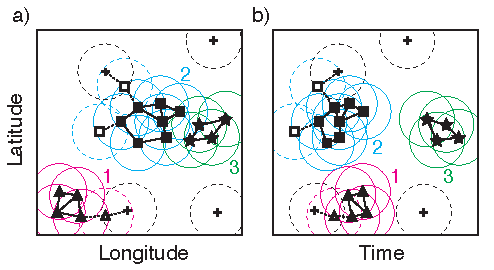
\includegraphics[scale=1]{GEC/Figures/dbscan.pdf}
    \caption{DBSCAN clustering example, with $minPts = 3$, showing the same clusters located in a) latitude and longitude and b) latitude and time.
    		 Solid rings show the $\epsilon$ distance from core points (filled), dashed rings are for non-core points (unfilled).
		 Triangles (1), squares (2), and stars (3) show clustered points, crosses are non-clustered points.}
    \label{gec:fig:dbscan}
 \end{figure}

WWLLN lightning strokes are separated by three dimensions: latitude, longitude, and time.
With time as a consideration two clusters that appear to overlap in Figure~\ref{gec:fig:dbscan}a, group~2 (blue) and group~3 (green), are separated by $\epsilon$ in time and are distinct groups as seen in Figure~\ref{gec:fig:dbscan}b.
DBSCAN is a physically realistic algorithm for clustering lightning data, such as WWLLN data, as the core points of a thunderstorm are the intense lightning centers while edge points are clustered but do not connect disparate lightning centers.

\subsection{Clustering WWLLN}

Accurate thunderstorm clustering of WWLLN data requires optimizing the clustering parameters $\epsilon$ and $minPts$.
WWLLN requires a second $\epsilon$ parameter, $\epsilon_{time}$, for clustering in time.
The parameter $\epsilon$ corresponds to the physical extent of an average thunderstorm, $\epsilon_{time}$ the duration, and $minPts$ the number of lightning strokes necessary to consider a thunderstorm electrically active.

As the clustering parameters are varied the total number of thunderstorms, the average thunderstorm area, and the average thunderstorm duration change.
In Figure~\ref{gec:fig:parameters}a it can be seen that $\epsilon$ has a high degree of control over thunderstorm area and total thunderstorms.
To balance the total number of thunderstorms, average area (320~km$^2$), and percentage of strokes clustered (89\%, not shown) the best value is found to be $\epsilon = 0.12^\circ$ or about 13~km.
To prevent consecutive thunderstorms from being clustered (e.g. one thunderstorm occurring in the same area as a previous distinct thunderstorm storm) $\epsilon_{time}$, Figure~\ref{gec:fig:parameters}b, needs to be smaller than average duration of a thunderstorm.
With this requirement the value of $\epsilon_{time} = 18$~minutes is found, giving an average thunderstorm cluster duration of 16~minutes.
The minimum number of strokes needed to produce a cluster is set at $minPts = 2$, as two detected WWLLN strokes confirms the presence of a thunderstorm.
A sharp drop in the total number of thunderstorms can be seen in Figure~\ref{gec:fig:parameters}c when $minPts$ moves from 2 to 3.
To get a majority of strokes included in the thunderstorm clusters while retaining reasonable physical attributes of the thunderstorms the parameters $\epsilon = 0.12^\circ$, $\epsilon_{time} = 18$~minutes, and $minPts = 2$~strokes were chosen.

 \begin{figure}[ht!]
    \centering
    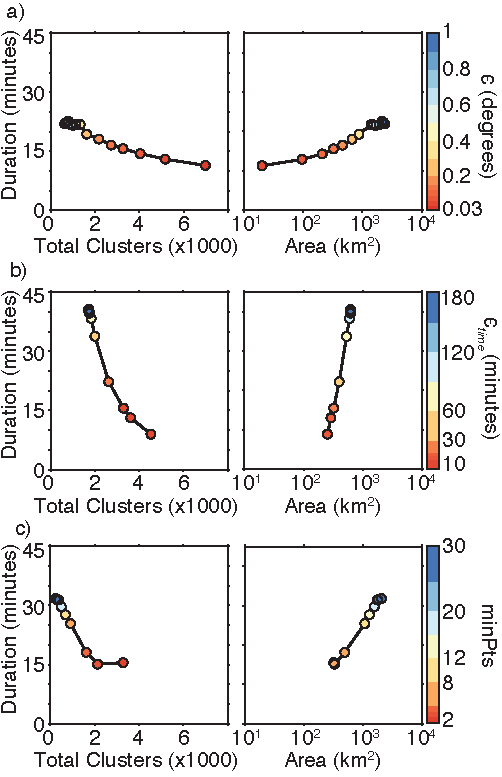
\includegraphics[scale=1]{GEC/Figures/parameters.pdf}
    \caption{Variation in average thunderstorm duration (rows), counts (left column) and area (right column) through varying one clustering parameter with the others held constant (constant set: $\epsilon = 0.12^\circ$, $\epsilon_{time} = 18$~minutes, and $minPts = 2$).
    		 a) $\epsilon$ varies from $0.03^\circ$ -- $1^\circ$.
		 b) $\epsilon_{time}$ varies from 10 -- 180 minutes.
		 c) $minPts$ varies from 2 -- 30 strokes.
		 }
    \label{gec:fig:parameters}
 \end{figure}

\section{WWLLN thunderstorm clusters}

Using the DBSCAN algorithm, the individual WWLLN lightning strokes from 2010 June - 2013 June are clustered into active thunderstorms.
Clustered WWLLN strokes allow for simple thunderstorm tracking as shown in Figure~\ref{gec:fig:evolution}.
Here the strokes comprising a thunderstorm are outlined with polygons every hour, and plotted with opacity increasing with time.
Figure~\ref{gec:fig:evolution} shows several active thunderstorms on 2013 May 21, 12 -- 23 UTC.
For clarity clustered thunderstorms with less than 50 strokes were removed from the plot.
The thunderstorm opacity increases at 8\% per hour with each color corresponding to a single thunderstorm cluster.

 \begin{figure}[ht!]
    \centering
    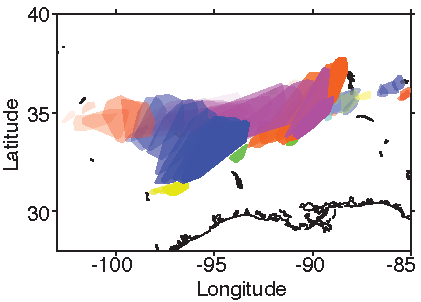
\includegraphics[scale=1]{GEC/Figures/evolution.pdf}
    \caption{Thunderstorm evolution from 2013 May 21, 12 -- 23 UTC.
    		 Polygons outline active lightning regions, colors correspond to thunderstorm cluster, opacity increases 8\%/hour.
		 For clarity, thunderstorms with less than 50 strokes were removed.}
    \label{gec:fig:evolution}
 \end{figure}

The cluster results can be directly compared to active precipitation regions as seen by the TRMM Precipitation Radar \citep{Kawanishi2000}.
Rainfall rates from the TRMM data product 2A25 were used as binned rates on a $0.25^\circ$ grid.
In Figure~\ref{gec:fig:overpass} the TRMM rainfall data are shown as the background image, gray areas are not in view of the satellite.
WWLLN strokes are shown in Figure~\ref{gec:fig:overpass} if they occur between the start and end times of the TRMM regional overpass.

 \begin{figure}[ht!]
    \centering
    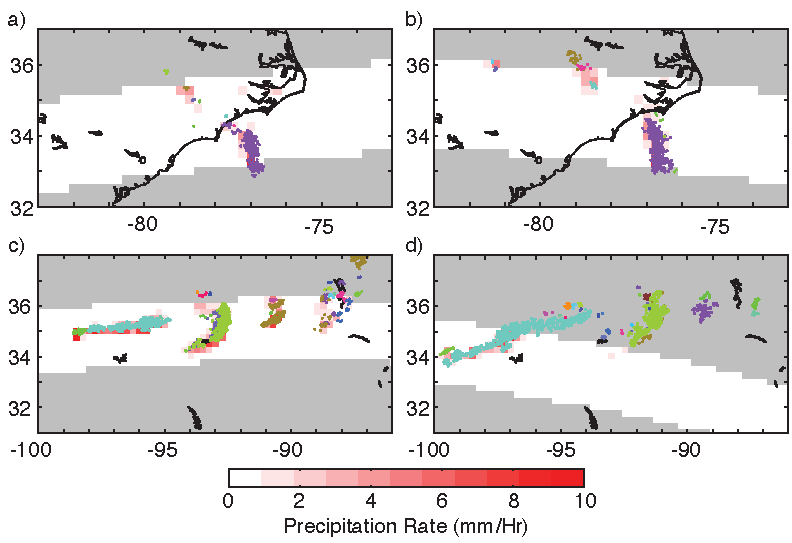
\includegraphics[scale=1]{GEC/Figures/overpass.pdf}
    \caption{WWLLN thunderstorm clusters (identified by color) over TRMM precipitation rate (mm/Hr) for 2013 May 06, 15:49 -- 15:59 UTC (a), 17:28 -- 17:37 UTC (b), 2013 May 21, 10:04 -- 10:13 UTC (c), 11:42 -- 11:52 (d).
    		(a) and (b) are successive passes as are (c) and (d), cluster colors are contiguous between passes.
		Gray areas were outside the range of the TRMM radar.}
    \label{gec:fig:overpass}
 \end{figure}

In Figure~\ref{gec:fig:overpass} two sets of consecutive overpasses are used, the first on 2013 May 06 from 15:49 -- 15:59 UTC (\ref{gec:fig:overpass}a) and 17:28 -- 17:37 UTC (\ref{gec:fig:overpass}b), the second in on 2013 May 21 from 10:04 -- 10:13 UTC (\ref{gec:fig:overpass}c) to 11:42 -- 11:52 UTC (\ref{gec:fig:overpass}d).
These passes were selected as they passed over the same thunderstorms twice with an appreciable amount of lightning activity in view of the satellite.
Unlike Figure~\ref{gec:fig:evolution}, the clustered WWLLN strokes are shown as individual strokes in the thunderstorm with many of the strokes overlapping each other in the center of the clustered regions.
The clustered thunderstorms match up well with the TRMM precipitation regions and clearly track the same thunderstorm between the consecutive overpasses.
Thunderstorms continue, and are clustered by WWLLN, well after TRMM no longer observes the area (green thunderstorm in Figure~\ref{gec:fig:overpass}c and~\ref{gec:fig:overpass}d).
There were no previous or later TRMM overpasses of these thunderstorms.

\section{Global thunderstorm activity}

Original estimates of global thunderstorm activity show afternoon peaks in lightning activity for each of the major lightning chimney regions: the Americas, Africa/Europe, and Asia \citep{Wilson1921}.
The global averaged WWLLN thunderstorm clusters show the previously measured long term averaged diurnal behavior of the global electric circuit activity, with a diurnal variation of 36\%.
The three year average of thunderstorm activity is shown in Figure~\ref{gec:fig:carnegie} for different regions (\ref{gec:fig:carnegie}a), for thunderstorm type (\ref{gec:fig:carnegie}b), and for seasons (\ref{gec:fig:carnegie}c), with the global average displayed in each panel (black).
Averages of thunderstorm activity are calculated from the total number of unique thunderstorms every 30~minutes.

 \begin{figure}[ht!]
    \centering
     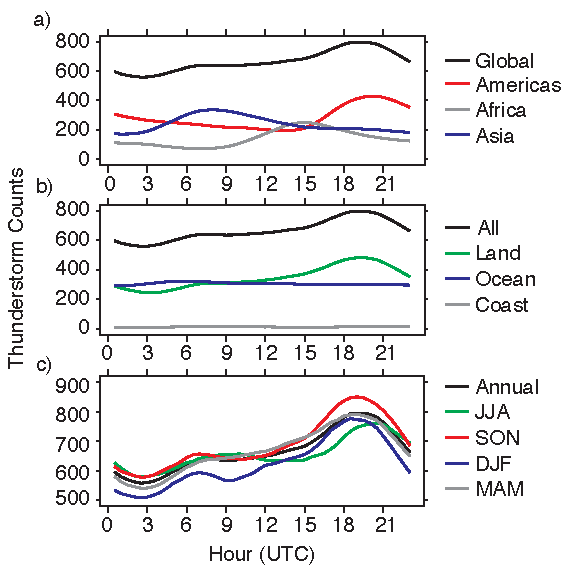
\includegraphics[scale=1]{GEC/Figures/carnegie.pdf}
    \caption{Diurnal variation of WWLLN thunderstorm 30~minute counts for 2010 -- 2013 obtained using the DBSCAN clustering algorithm.
    		 For a) thunderstorms over each major lightning chimney region (divided between longitudes $-180^\circ$, $-30^\circ$, and $60^\circ$),
		 b) all, land, ocean, and coastal thunderstorms (coastal thunderstorms have strokes over land and ocean),
		 and c) the full year and each season.
		 }
    \label{gec:fig:carnegie}
 \end{figure}

Each chimney region is separated in Figure~\ref{gec:fig:carnegie}a with peaks in thunderstorm activity occurring in the local afternoon (Americas 19~UTC, Africa 15~UTC, and Asia 8~UTC) with a slow decrease during the night until a minimum in the early hours of the morning.
A strong diurnal variation is evident for thunderstorms over land, seen in Figure~\ref{gec:fig:carnegie}b, with  little diurnal variation in oceanic thunderstorm activity.
On average WWLLN observes a total of $660 \pm 70$ thunderstorms on any given day of the year.
While the total is lower than previous estimates in the 1000 -- 2000 thunderstorm range, those estimates were made using partial or extrapolated datasets.
For each chimney region the average number of thunderstorms are $280 \pm 80$ for the Americas, $140 \pm 60$ for African and Europe, and $240 \pm 50$ for Asia and the Maritime Continent.
The long-term thunderstorm behavior observed by WWLLN resembles the previous measurement of global electric circuit behavior.
Of the clustered thunderstorms $350 \pm 70$ were continental and $300 \pm 10$ were oceanic.
This is in contrast to the disparity in the distribution of individual lightning strokes where a majority are continental; the continental thunderstorms tend to be larger with higher stroke rates than those over the oceans.

There are slight changes in the overall diurnal behavior between each season shown Figure~\ref{gec:fig:carnegie}c.
The contribution of each chimney region, divided by northern and southern hemisphere, is shown in Figure~\ref{gec:fig:bimonthly}.
The overall seasonal change in thunderstorm activity is clearly seen with the change in dominant contributor from the northern hemisphere in May -- August to the southern hemisphere in November -- February.
In the shoulder seasons (March -- April and September -- October) the different chimneys are closer in activity levels to each other.
The shift in peak activity times for each chimney region between northern and southern summer reflects the difference in longitudinal landmass distribution of each region.
For example the North America peak occurs at 23:30 UTC while the South America peak occurs at 18:30 UTC since the South American lightning regions are, in general, farther east than the North American ones.
This time change in regional contributions has been seen in other global circuit measurements; in the Vostok, Antarctica electric field measurements of the fair weather field peak changes from 18:00 UTC in January to 21:00 UTC in August \citep{Burns2005, Burns2012}.

 \begin{figure}[ht!]
    \centering
    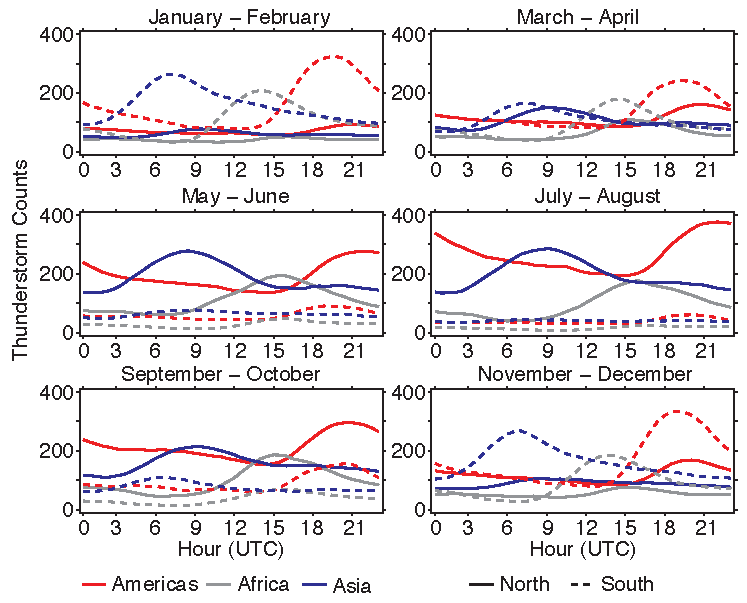
\includegraphics[scale=1]{GEC/Figures/bimonthly.pdf}
    \caption{Diurnal variation of WWLLN thunderstorms for each major chimney region (colors) divided by hemisphere (Northern Hemisphere solid line, Southern Hemisphere dashed line).
    		Each panel shows two months of thunderstorm clusters averaged over 2010 -- 2013.
		 }
    \label{gec:fig:bimonthly}
 \end{figure}

\section{Temporal thunderstorm activity}

As a result of constantly growing number of WWLLN stations, the number of WWLLN strokes detected increases with time due to improvements in the network and the detection efficiency.
As a result long term tracking of stroke rate  cannot be used without deconvolving detection efficiency improvements.
However thunderstorm counts have remained relatively constant while stroke rate has increased; WWLLN has been capable of detecting almost every thunderstorm since 2005 \citep{Jacobson2006c}.
In Figure~\ref{gec:fig:timescale}a the daily average 30~minute thunderstorm counts (black) are plotted alongside the daily average stroke rate (red).
It can been seen that the stroke rate has increased relatively steadily while the thunderstorm count has remained relatively stable.

 \begin{figure}[ht!]
    \centering
    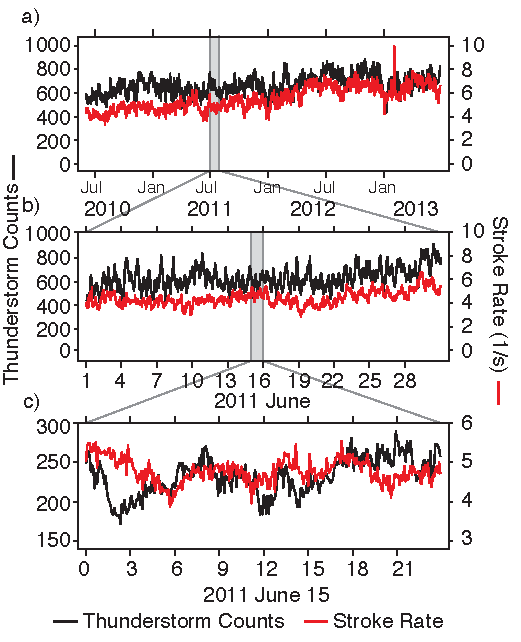
\includegraphics[scale=1]{GEC/Figures/timescale.pdf}
    \caption{Variation in WWLLN thunderstorm count (black) and stroke rate (red) for:
    		a) daily averages 30~minute counts from 2010 June -- 2013 June,
		b) 30~minute counts from 2011 June 01 -- 30,
		c) 5~minute counts from 2011 June 15, 00 -- 23 UTC.}
    \label{gec:fig:timescale}
 \end{figure}

The daily average thunderstorm count remains relatively constant during 2010 -- 2013, while the stroke rate increases during the same time span.
The thunderstorm count increased an average of 3\% per year, while the stroke had a much higher yearly increase of 13\%.
Similarly 90\% of the daily thunderstorm averages are within 20\% of the mean for the three years.
Previous work has suggested that changes in climate will cause a change in global thunderstorm behavior \citep{Williams2005a, Price2009a}.
During 2010 -- 2013 the average global surface temperature and thunderstorm count have both remained relatively constant \citep{Hansen2013a}, but future changes in global temperature may be reflected in the global average thunderstorm count.

Figure~\ref{gec:fig:averaging} shows that the typical diurnal behavior of Figure~\ref{gec:fig:carnegie} emerges only after long term averaging.
When examining the thunderstorm counts on a monthly scale (Figure~\ref{gec:fig:averaging}, dot-dash line) the long term average begins to emerge, while over a single day (Figure~\ref{gec:fig:averaging}, dashed line), the expected diurnal behavior is missing.
Similarly, on the daily scale of Figure~\ref{gec:fig:timescale}c it can be seen clearly that stroke rate does not follow thunderstorm counts as located by WWLLN.
Despite the short time scale variation, the overall average of the data still accurately reproduces the expected global thunderstorm activity in Figure~\ref{gec:fig:carnegie}.
With such short time scale variations global observations of the global electric circuit source mechanism, be it with ground lightning networks or several geostationary satellites, need to occur along with an accurate measure of the return current to better understand the charging of the global electric circuit.

 \begin{figure}[ht!]
    \centering
    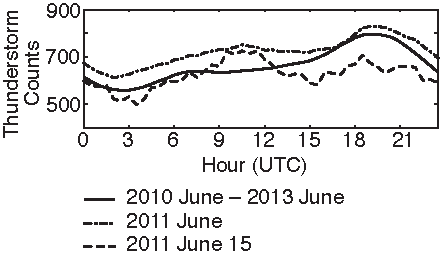
\includegraphics[scale=1]{GEC/Figures/averaging.pdf}
    \caption{Diurnal UTC variation in WWLLN 30~minute thunderstorm count for:
    		multi-year average of Figure~\ref{gec:fig:timescale}a (solid line),
		monthly average of Figure~\ref{gec:fig:timescale}b (dot-dash line),
		and 30~minute averages of Figure~\ref{gec:fig:timescale}c (dashed line).}
    \label{gec:fig:averaging}
 \end{figure}

\section{Global Electric Circuit Thunderstorm Contribution}

With the WWLLN thunderstorm clusters, a simple model is made to estimate the total contribution of thunderstorms and electrified storm clouds to the global electric circuit.
\citet{Mach2011} considered LIS/OTD observed land thunderstorms with less than 1.7 flashes min$^{-1}$ and ocean thunderstorms with less than 0.33 flashes min$^{-1}$ electrified storm clouds.
For an average storm duration of 15~minutes these cutoffs are 26 flashes for land and 5 flashes for oceanic electrified storm clouds (ESCs).
With a WWLLN-LIS/OTD detection efficiency of 6.4\% over land and 17\% over oceans \citep{Rudlosky2013}, WWLLN would expect cutoffs of 2~strokes per thunderstorm over land and 1~stroke per thunderstorm over oceans.
Given the clustering parameters used in this work requires a minimum of 2~strokes to be considered a thunderstorm, every un-clustered WWLLN stroke is considered a single ESC.
The daily average of thunderstorms and ESCs observed by WWLLN are shown in Figure~\ref{gec:fig:wilson}a.
Since not all ESC will produce lightning the counts shown in Figure~\ref{gec:fig:wilson}a should be considered a low estimate.

  \begin{figure}[ht!]
    \centering
    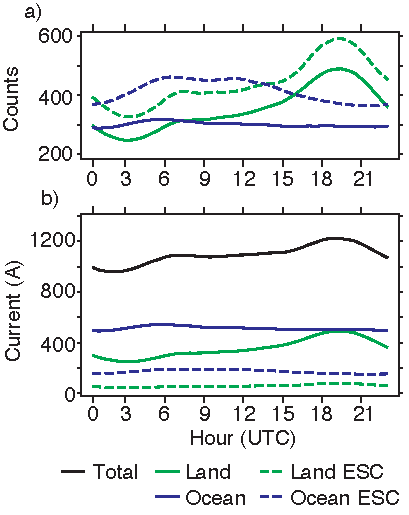
\includegraphics[scale=1]{GEC/Figures/wilson.pdf}
    \caption{A simple model of the total global electric circuit current with contributions from land thunderstorms (green solid), oceanic thunderstorms (blue solid), land electrified storm clouds (green dashed), and oceanic electrified storm clouds (blue dashed).
    		a) shows the counts for each group and b) the current contribution to the total (black line).
		}
    \label{gec:fig:wilson}
 \end{figure}

The average thunderstorm and ESC current contribution is taken from the overflight data of \citet{Mach2010}.
Average current contribution for land thunderstorms is 1.0~A, for oceanic thunderstorms 1.7~A, for land ESCs 0.41~A, and for oceanic ESCs 0.13~A.
The total current for each contributor and the total current is shown in Figure~\ref{gec:fig:wilson}b.
The average thunderstorm current is found to be $1090 \pm 70$~A with a total peak-to-peak variability of 24\%.
The largest contributor are oceanic thunderstorms (47\%) with $510 \pm 10$~A, followed by land thunderstorms (32\%) with $350 \pm 70$~A.
Overall ESCs contribute 21\% to the thunderstorm global circuit current.

With a similar model based on the TRMM LIS/OTD data, \citet{Mach2011} found ocean thunderstorms contribute 32\% and land thunderstorms 55\%, with a total ESC contribution of 13\% to the total mean current of 2.04~kA.
Their difference in current and contributor fraction stems from an increased count of land thunderstorms.
This highlights a shortcoming of this simple model, land thunderstorms tend to be larger than oceanic storms; thunderstorm area should be taken into account along with overall counts.
However to validate any global circuit model a comparison needs to be made with simultaneous fair weather return current measurements in order to constrain the models.

\section{Conclusion}

Global thunderstorm count is a good measure of global electric circuit activity and for a simple model of the circuit; the location and size of thunderstorms is necessary along with totals to create a more accurate model of the real time fair weather return current.
WWLLN strokes are successfully clustered into thunderstorms using the DBSCAN clustering algorithm with appropriately chosen clustering parameters.
The clustered thunderstorms were compared against the TRMM Precipitation Radar and a case study of thunderstorm tracking and evolution.
When the three years of WWLLN data were averaged the diurnal behavior of global thunderstorm activity aligned with the expected behavior of both thunderstorms and the fair weather return current.
The results of global thunderstorm and electrified storm cloud activity are combined with upward thunderstorm current averages to create an estimate of the fair weather return current.
The model found an average thunderstorm current contribution of $1090 \pm 70$~A.
This, and future, estimates of the current can be validated against an accurate fair weather return current measurement.

\subsection*{Acknowledgments}
The TRMM data used in this effort were acquired as part of the activities of NASA's Science Mission Directorate, and are archived and distributed by the Goddard Earth Sciences (GES) Data and Information Services Center (DISC).
